
%% Estructura principal para un reporte de Trabajos intersemanales CIRCAE %%
%% Autor: Edison Abado Ancco

\documentclass[a4paper]{article} %tamaño del papel y el tipo de transcripción que será IEEE
%\usepackage{geometry}
\usepackage[top=1.8cm,bottom=1.8cm,left=1.8cm,right=1.8cm,headsep=8pt,a4paper]{geometry}
%\usepackage[total={6.5in,10in},left=1in,top=0.5in,includehead,includefoot]{geometry}
\usepackage[utf8]{inputenc} %el tipo de codificación que incluye símbolos como la tilde
\usepackage[spanish]{babel} % hacemos que nuestro documentación vaya en español
\usepackage{cite} % citas bibliográficas
\usepackage{graphicx} %gráficos, usaremos solo .jpg o .png con estándares que ya veremos
%\usepackage{subfigure} %usar subfiguras
\usepackage{url} %agregar direcciones url
\usepackage{amsmath} %expresiones matemáticas
\newtheorem{teor}{Teorema}[section] %definimos la enumeración de Teoremas usando la etiqueta \begin{teor} ... \end{teor} para los ejemplos, podemos darle etiquetas para referenciarlas a lo largo del texto
\newtheorem{ejem}{Ejemplo}[section] %definimos la enumeración de Ejemplos usando la etiqueta \begin{ejem} ... \end{ejem} para los ejemplos, podemos darle etiquetas para referenciarlas a lo largo del texto
\newtheorem{exper}{Experimento}[section] %definimos la enumeración de Ejemplos usando la etiqueta \begin{exper} ... \end{exper} para los Experimentos, podemos darle etiquetas para referenciarlas a lo largo del texto
\usepackage{setspace} %LA usamos para asignar el interlineado
%%%%%%% settings para incluir codigo fuente en cualquier lenguaje
\usepackage{listings} %comenzamos la configuración de nuestras lineas de codigo que se incluirá de ser necesario en el documento
\usepackage[usenames]{color} %seteamos el uso de nombre y color
\definecolor{gray97}{gray}{.97}%definimos nombre y color
\usepackage{textcomp}
\usepackage{tikz,bm}
\usetikzlibrary{calc, positioning, shapes, backgrounds, fit, arrows}
\usepackage{tikz,bm}
\usepackage[raggedrightboxes]{ragged2e}
\usepackage{pgf-spectra}

\usepackage{siunitx}

\usepackage{contour}
\lstset{
	frame=Ltb,
	framerule=1pt,
	framextopmargin=5pt, %margen de arriba
	framexbottommargin=5pt, %margen de abajo
	framexleftmargin= -2pt, %separacion del margen izquierdo
	framesep=2pt,
	rulesep=0.2pt,
	backgroundcolor=\color{gray97},
	rulesepcolor=,
	tabsize=4,
	rulecolor=\color[RGB]{106, 182, 217}, %AZUL
	upquote=true,
	aboveskip={1.5\baselineskip}, %despues de la linea de texto
	columns=fixed,
	showstringspaces=false,
	extendedchars=true,
	breaklines=true,
	prebreak = \raisebox{0ex}[0ex][0ex]{\ensuremath{\hookleftarrow}},
	showtabs=false,
	showspaces=false,
	showstringspaces=false,
	basicstyle=\scriptsize\ttfamily\color[RGB]{39, 100, 46}, %Numeros de lineas, simbolos, puntos y coma y demas
	identifierstyle=\ttfamily\color[RGB]{56, 140, 189}, %variables
	commentstyle=\color[RGB]{62, 179, 101}, %comentarios
	stringstyle=\color[RGB]{247, 165, 42}, %impresiones
	keywordstyle=\bfseries\color[RGB]{237, 118, 150}, %funciones
	%
	numbers=left,
	numbersep=6pt, %separacion del numero
	numberstyle=\tiny,
	numberfirstline = false,
	breaklines=true,
}
\usepackage{graphicx}
\usepackage[colorinlistoftodos]{todonotes}
%%%%%%%
\providecommand{\keywords}[1]{\textbf{\textit{Términos Clave---}} #1}

\usepackage{hyperref}
\usepackage{wrapfig}
\usepackage{caption}
\usepackage{subcaption}
\usepackage{circuitikz}

\usepackage{float}
\title{
	\textsc{Universidad Nacional de San Antonio Abad del Cusco}\\
	\textbf{Compuertas Lógicas}\\
	Preinforme 1}

\author{
	\begin{tabular}{lr}
		Edison \textsc{Abado Ancco} & 145012 \\
	\end{tabular}
}


\begin{document}
	\begin{titlepage}
		\newcommand{\HRule}{\rule{\linewidth}{0.5mm}} 
		\center
		\textsc{\LARGE \vspace{1.1cm} \\ Universidad Nacional de San \\[0.2cm] Antonio Abad del Cusco}\\[1.2cm] 
		
\includegraphics[width=4cm]{IMAGENES/logoLiC}\\[1cm]
		\textsc{\Large Facultad de Ingeniería Eléctrica, \\ Electrónica, Informática y Mecánica}\\[0.5cm] 
		\textsc{\large Escuela Profesional de Ingeniería Electrónica}\\[0.5cm]
		\textsc{\Large \textbf{Circuitos Electrónicos II}}\\[0.5cm] 
%		\textsc{\huge Informe Final}\\[0.2cm]
		\HRule \\[0.4cm]
		{ \huge \bfseries Amplificador Diferencial con alguna aplicación}\\[0.30cm] 
		\HRule \\[1.4cm]
		\begin{minipage}{\textwidth}
			\center 
			
			\emph{Docente:} \\
			Prof. Franklin  \textsc{Cardeñoso Fernandez} \\[1cm]
			
			\begin{tabular}{c}
				\emph{Alumnos:}  \\
				Edison   \textsc{Abado Ancco} - 145012 \\
				Joseph \textsc{Garfias Quispe} - 554444 \\
				Alumno 3 \\
				Alumno 4 \\
				Alumno 5
			\end{tabular}
		\end{minipage}\\[2cm]
		\today
	\end{titlepage}
	
	
\newpage
	
%\tableofcontents indice bloqueado xD
	
\setlength{\parindent}{0pt} % Stop paragraph indentation
	


\section{Tecnologías de los CMOS y TTL}

Los diseños de los circuitos integrados están basados en el tipo de tecnología (TTL, CMOS, ECL, etc) que presenta que nos permita solucionar los problemas de los amplificadores operacionales y sus derivados, desde su propia arquitectura, ruido que presenta cada circuito al momento de diseñar e implementar en la realidad, es por eso, que se analizará el uso de los transistores BJT y CMOS.
	\begin{paragraph}{Transistores BJT}
		Dispositivo electrónico que tiene como función la de permitir el paso de corriente en un único sentido de manera controlada.
		\begin{figure}[H]
			\centering
			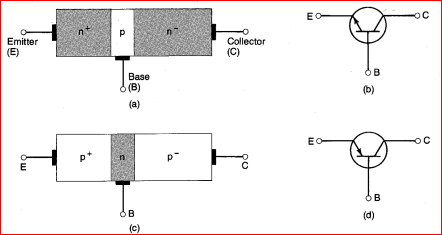
\includegraphics[width=7.5cm,height=4cm]{IMAGENES/1.PNG}
			\caption{Transistor BJT (a) NPN y (b) su símbolo y (c) PNP y (d) su símbolo. \cite{1}}
			\label{f_1}
		\end{figure}
	\end{paragraph}



	\begin{paragraph}{Transistores CMOS}
		La tecnología CMOS hace uso de básicamente de transistores de efecto de campo NMOS y PMOS, este tipo de ciencia es más rapida y consumo menos potencia de energía que requiere otras familias. Debido a que presenta mayor densidad de integración.  
		\begin{figure}[!h]
			\centering
			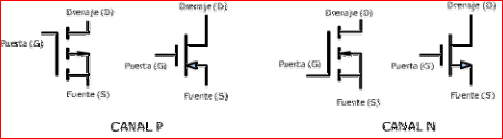
\includegraphics[width=7.5cm,height=4cm]{IMAGENES/2.PNG}
			\caption{Símbolos más comunes de los transistores PMOS y NMOS \cite{2}}
			\label{f_2}
		\end{figure}
	\end{paragraph}



	Las diferencias que presentan las familias de los CMOS y los TTLs son:
	\begin{itemize}
		\item Los CMOS presenta un mayor intervalo de voltaje y un factor de carga más elevado que los TTL.
		\item Los CMOS tienen una mayor inmunidad al ruido que los TTL.
		\item Los CMOS son más lentos en cuanto a velocidad de operación que los TTL.
		\item Los circuitos integrados CMOS es de menor consumo de potencia que los TTL.
		\item La inmunidad al ruido de CMOS es mucho mejor que los circuitos TTL.
	\end{itemize}


\section{Nuevas tecnologías}

	A lo largo de los años se empezaron a realizar estudios en los nanotubos de carbono (CNT) que presenta diferentes configuraciones, en especial en las nanométricas que están empezando a tener lugar importante en los amplificadores diferenciales, amplificadores operacionales entre otros derivados que son empleados en las tecnologías conocidas, así como en las telecomunicaciones.\\
	
	Las CNT se comportan como sistemas unidimensionales (1D) ya que sus dimensiones se encuentran en escalas nanométricas, que definen sus propiedades físicas especiales que presenta, cuyo parámetros eléctricos y ópticos son muy superiores a los semiconductores Si, Ge y GaAs.\\
	
	En la búsqueda de dispositivos cada vez más pequeños con bajo consumo de energía y alta velocidad, en ese sentido se vio como opción los derivados de los nanotubos de carbono, SWCNT (Nanotubos de carbono de pared simple) que presentan un comportamiento metálico o semiconductor que nos permite proyectae buenos hilos conductores y uniones P-N a escala nanométrica.


\subsection{Nanotransistores basados en CNT}

	Los transistores FET estan compuestos de dos electrodos metálicos (fuente y drenaje) conectados por un semiconductor. Al variar la anchura del canal, la tensión de polarización en el electrodo llamado "puerta" controla el flujo de corriente entre la fuente y drenaje.\\
	
	En \cite{3} menciona que se demostró que los CNT se podian utilizarse en los diseños de FET. Donde los nanotubos de carbono se encuentra la parte superior, interconectando asi los dos electrodos de metales nobles.
	\begin{figure}[H] 
		\centering
		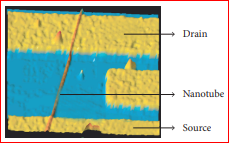
\includegraphics[width=0.25\textwidth]{IMAGENES/3.PNG}
		\caption{Imagen de transistor de efecto de campo con CNT obtenida por microscopio de fuerza atómica  \cite{3}}
		\label{f_3}
	\end{figure}
	
	



	\bibliographystyle{ieeetr}
	\bibliography{bibliografia}



%%%%%%%%%%%%%%%%%%%%%%%%%%%%%%5
%% BIBLIOGRAFÍA %%%
%%%%%%%%%%%%%%%%%%%%%%%%%%%%%%%



	
	
\end{document}
